\section{Ergebnis} % (fold)
\label{sec:ergebnis}
	Bereits zu Beginn des Projekts war es wichtig es messbar zu machen. Dafür wurde eine Testumgebung aufgebaut, mit deren Hilfe die Seite nach ihrer Geschwindigkeit getestet werden kann. Ganz entscheidend war dabei die Webpagetest API in Verbindung mit Google Spreadsheets. Damit lassen sich regelmäßig automatisierte Tests durchführen und die Daten werden nach erfolgreichem Test automatisch in einer Spreadsheet Tabelle gespeichert. Die über den Zeitraum der Arbeit hinweig gesammelten Daten sind hier finden: \url{http://tinyurl.com/l5usz79}. Diese Daten wurden anschließend mittels \url{http://Chartjs.org} in Diagrammen aufbereitet und alle Diagramme sind auch Online abrufbar unter: \url{http://bithugger.github.io/bachelorthesis/}

	\subsection{Wie wurde getestet?} % (fold)
	\label{sub:wie_wurde_getestet}
		Damit mittels Google Spreadsheets die Webpagetest API verwendet werden kann, ist es nötig einen sogenannten API-Key anzufordern. Ein solcher Key ist kostenlos unter der Adresse: \url{http://www.webpagetest.org/getkey.php} zu erhalten und bietet die Möglichkeit täglich 200 Seitenaufrufe zu tätigen. Als Seitenaufruf zählt sowohl die "`first view"' als auch "`repeat view"'. Die Tests sind 30 Tage abrufbar und gespeichert.\\

		Für das Testen der Seite kann aus einer Vielzahl an Teststandorten gewählt werden. Damit lässt sich nachvollziehen wie beispielsweise die Ladezeiten aus der USA oder Asien sind. Je nach Zielgruppe sollten Tests von verschiedenen Standorten in betracht gezogen werden.\footnote{Eine volle Liste der zur Verfügung stehenden Teststandorte ist im Anhang unter Punkt: \ref{sub:webpagetest_teststandorte} zu finden.} Für dieses Projekt wurden ausschließlich Teststandorte aus der USA und Europa gewählt.\\

		Als Testparameter wurde eine Anzahl von 9 Tests pro Testlauf gewählt. Dabei wurde sowohl die "`first view"' als auch die "`repeat view"' aufgezeichnet. Von den 9 Testläufen wurde der Median als Ergebnis des Testlaufs verwendet. Über den Zeitraum der Arbeit wurde die Seite 1089 Tests unterzogen.\\

		Das größte Problem bestand in der möglichst genauen Messzeiterfassung für die Ladezeiten mittels Smartphone. Webpagetest stellt nur einen Smartphones Teststandort in Dulles USA zu Verfügung. Da die Latenz zwischen dem Hosting in Deutschland und dem Seitenaufruf in der USA sehr viel größer ist, als wenn dieser direkt aus Deutschland erfolgt, wurde nach einer Lösung gesucht diese Messungen exakter zu gestalten.
		Die Lösung dafür ist, ein zweites Hosting mit der selben Seite in den USA zu erstellen. Dafür wurde die "`Microsoft Azure Cloud"' verwendet. Eine kostenlose Testversion ermöglicht es, ganz einfach auf verschiedensten Kontinenten eine Webseite zu hosten. Die Seite wurde für die Tests Online geschaltet und nach den Testläufen wieder Offline genommen.

	% subsection wie_wurde_getestet (end)

	\subsection{Datenauswertung}
	\label{sub:datenauswertung}
		Folgende Daten wurden bei jedem Testlauf erfasst:

		\begin{itemize}
			\item Speed Index
			\item TTFB (ms)
			\item Render start (ms)
			\item Visually complete (ms)
			\item Dom Content loaded (ms)
			\item Site fully loaded (ms)
			\item Requests
			\item Bytes in Document
		\end{itemize}

		\begin{figure}[htbp]
			\begin{center}
				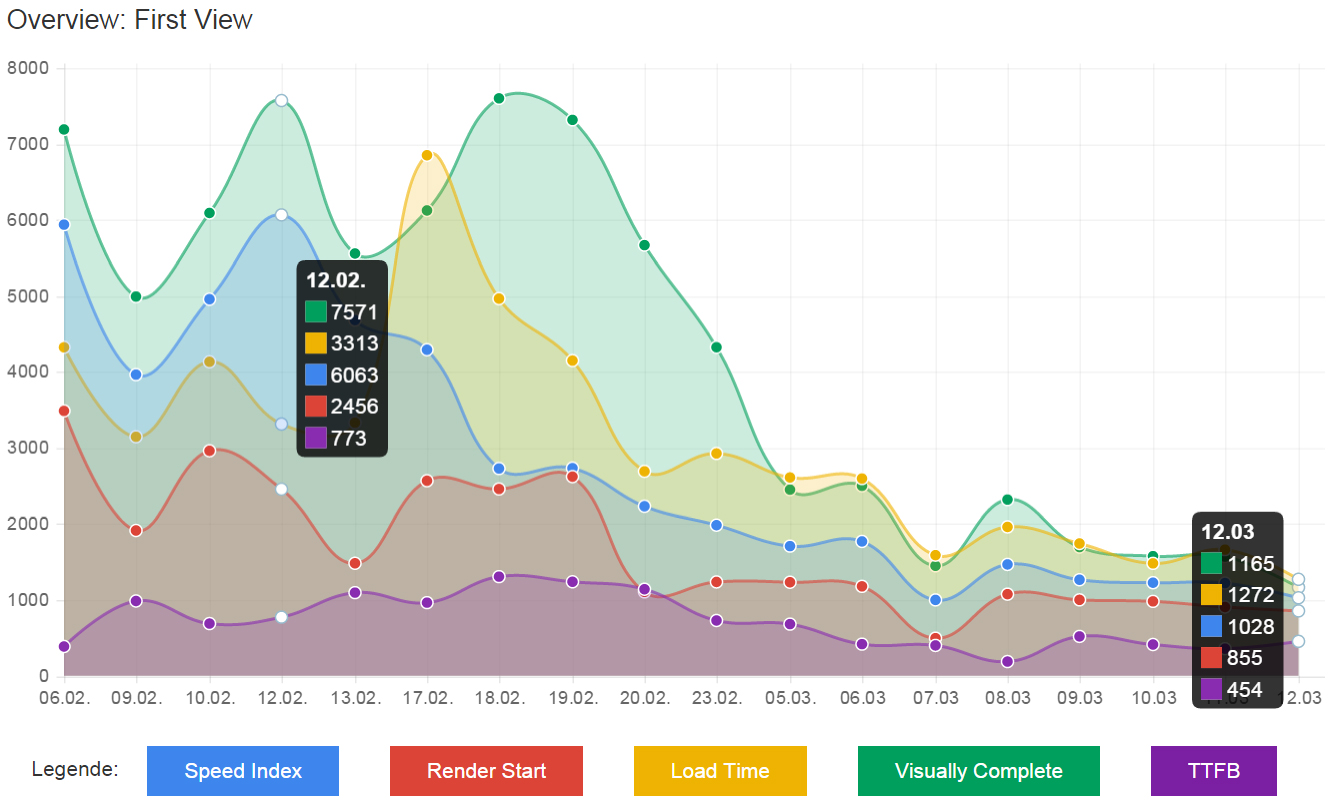
\includegraphics[width=\textwidth]{data_all.jpg}
				\caption{Datenauswertung - Überblick }
				\label{fig:data_all}
			\end{center}
		\end{figure}

		\begin{figure}[htbp]
			\begin{center}
				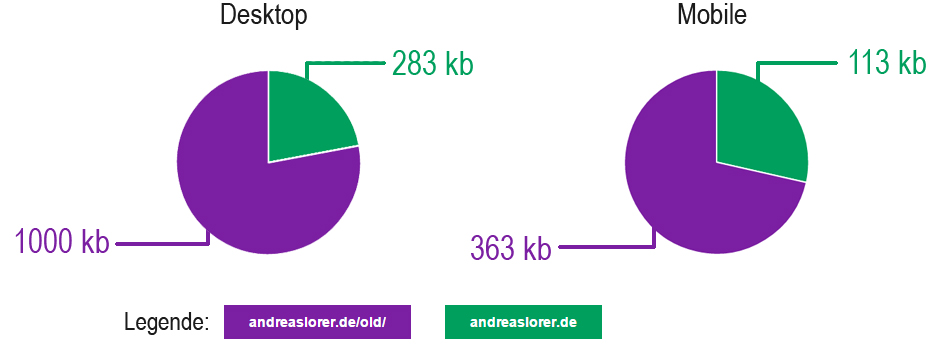
\includegraphics[width=\textwidth]{site_size_in_kb.jpg}
				\caption{Seitengröße in Kilobyte}
				\label{fig:site_size_in_kb}
			\end{center}
		\end{figure}

		\begin{figure}[htbp]
			\begin{center}
				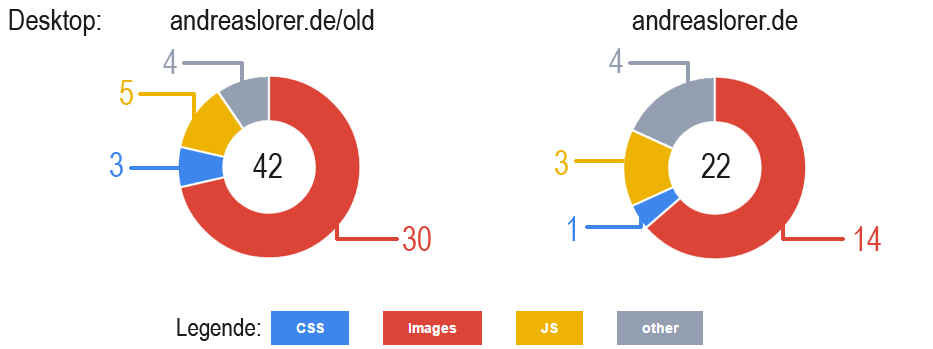
\includegraphics[width=\textwidth]{amount_of_requests.jpg}
				\caption{Anzahl an Requests via Desktop}
				\label{fig:amount_of_requests}
			\end{center}
		\end{figure}	

		\begin{figure}[htbp]
				\begin{center}
					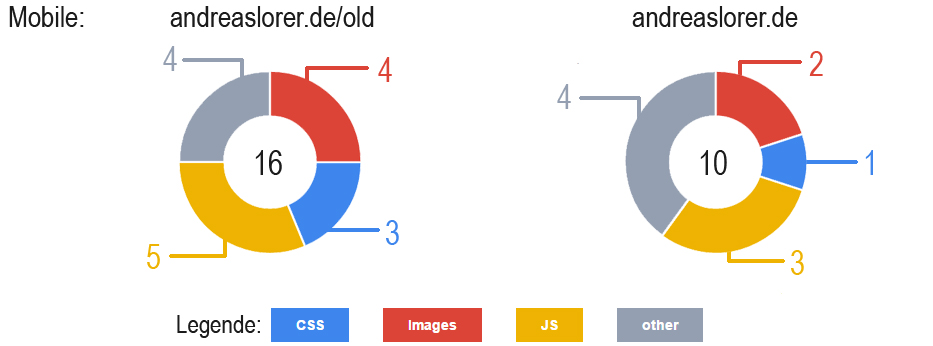
\includegraphics[width=\textwidth]{amount_of_requests_mobile.jpg}
					\caption{Anzahl an Requests via Mobile}
					\label{fig:amount_of_requests_mobile}
				\end{center}
			\end{figure}
			
				

	% subsection datenauswertung (end)
% section ergebnis (end)

\pagebreak
